\chapter{Design}
\section{Layer}
Si pensi alla simulazione come se fosse un micro-mondo, una ``città'' complessa
e ricca di informazioni. È di interesse capire il livello di temperatura oppure di inquinamento nelle varie aree cittadine, dati invisibili
all'occhio umano ma comunque presenti nell'ambiente e percepibili da chi lo abita. Si ha bisogno
di inserire nell'ambiente degli ``strati'' invisibili che hanno il compito di raccogliere queste informazioni.
È possibile, in Alchemist, definire questi ``strati'' di dati, chiamati Layer.
\newline
Nel contesto di questo progetto è stato necessario l'utilizzo di un Layer che avesse la funzione di ``rete di raccolta''
dei feromoni che, nella simulazione di riferimento\space\ref{refSim}, venivano rilasciati dalle tartarughe nelle varie posizioni
dello spazio. In questo caso il layer ha la stessa dimensione dell'ambiente, in modo tale da poter suddividere l'intera area nelle varie \textit{patch} di cui si 
è discusso sopra.
Il layer, chiamato \textit{PheromoneLayer} ha come compiti:
\begin{itemize}
    \item Implementare una struttura dati per tenere traccia della quantità di feromone presente in ogni posizione.
    \item Offrire un modo per aggiornare i valori del feromone.
    \item Condividere con le altre classi la struttura dati contenente la quantità di feromone per una specifica posizione.
    \item Lasciare la possibilità all'utente di decidere le dimensioni dell'area totale di riferimento e di ogni \textit{patch}.
\end{itemize}

\subsection{Le posizioni}
Un aspetto di particolare rilevanza è stato il processo decisionale relativo alla gestione delle posizioni collegate 
al deposito del feromone. Nella simulazione di riferimento\space\ref{refSim} si trova uno spazio a griglia, dove l'area totale è suddivisa
in ``micro-aree'' chiamate \textit{patch}. In Alchemist, tuttavia, non è presente il concetto di ``area'' o ``spazio'', necessario per individuare una \textit{patch},
in quanto le posizioni sono puntiformi e non necessariamente hanno coordinate intere. Il layer sviluppato ricalca l'area (rettangolare o quadrata) del sistema iniziale,
implementando anche un sistema di conversione che trasforma la posizione puntiforme in modo tale da emulare la presenza di una ``area'' bidimensionale, a forma di quadrato, che corrisponde alla \textit{patch}.
Entrambe le misure, ovvero quella della griglia e quella della \textit{patch} sono dinamiche e possono essere modificate dall'utente.

\begin{figure}[h!]
    \centering
    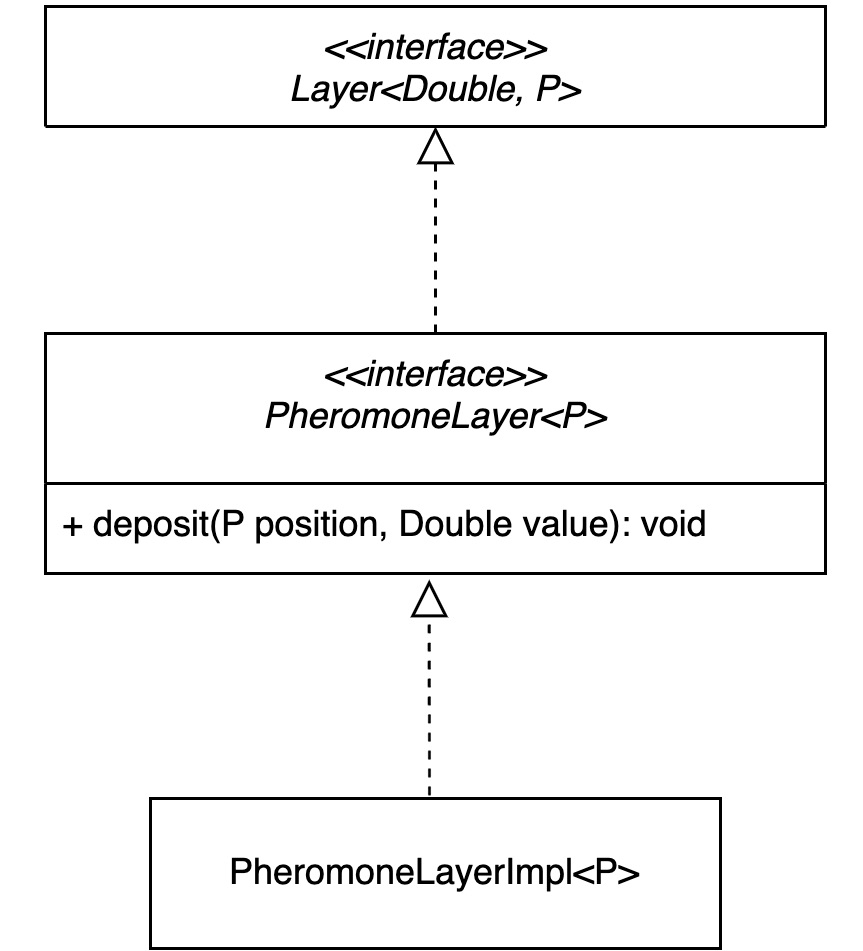
\includegraphics[width=.8\linewidth]{figures/pheromoneLayer.jpeg}
    \caption{Struttura PheromoneLayer}\label{fig:phLayer}
\end{figure}

\clearpage
\section{Le entità}
Una volta definito l'ambiente di simulazione è importante determinare la struttura e la logica delle 
entità che lo abiteranno. Nella simulazione di riferimento\space\ref{refSim} è possibile individuare come abitanti le tartarughe
che, muovendosi, rilasciano una traccia chimica chiamata ``feromone''. Dunque, concettualmente, la tartaruga è un ``contenitore'' infinito di 
feromoni e, muovendosi, ne rilascia una parte nell'ambiente. Alchemist possiede il concetto di nodo\space\ref{node} che, per definizione, 
è un contenitore di molecole che vive in un ambiente. È stato quindi necessario solamente definire la tipologia di molecola
appartenente al nodo per tradurre questo aspetto della simulazione (ma anche del mondo reale) in Alchemist.
\begin{figure}[h!]
    \centering
    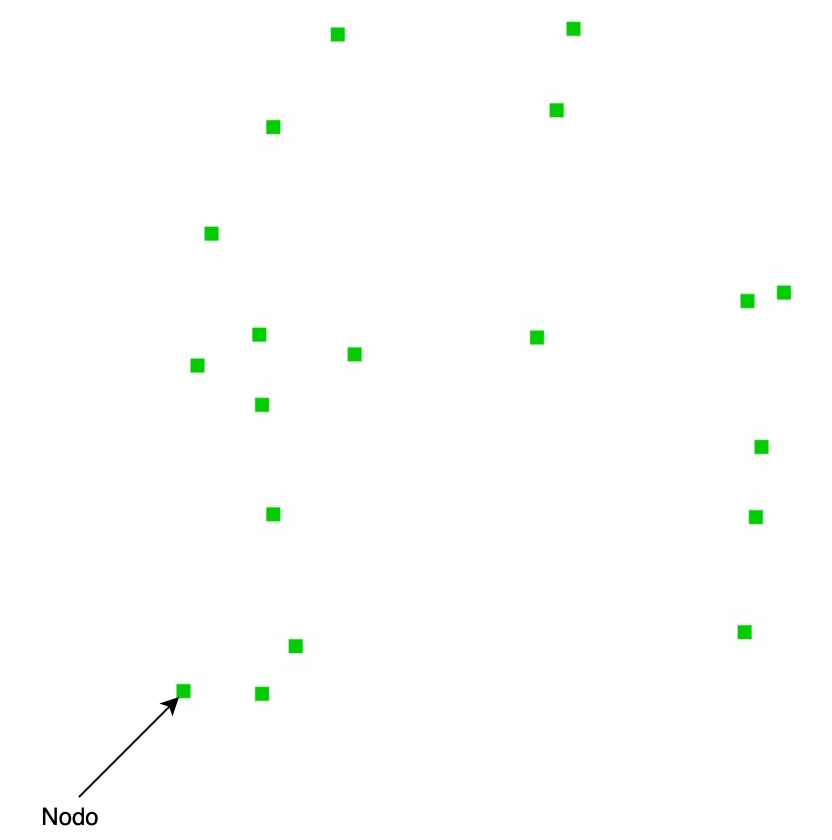
\includegraphics[width=.7\linewidth]{figures/nodes.png}
    \caption{Rappresentazione grafica dove ogni punto è un nodo}\label{fig:nodes}
\end{figure}
\clearpage
\section{Il movimento}

\section{Reazioni globali}
La Reazione Globale o \textit{Global Reaction} rappresenta uno strumento fondamentale per descrivere
le interazioni e i processi che avvengono all'interno di un sistema simulato.
Possono essere utilizzate per modellare una vasta gamma di fenomeni, dalla diffusione chimica alla dinamica dei sistemi biologici.
Contrariamente alle reazioni locali, le \textit{Global Reaction} hanno effetti concreti sull'intero contesto in esame. 
Realizzare una modellazione precisa e realistica di questi fenomeni può essere di grande interesse per indagare tutti i risultati possibili.. 
Nell'ambito di questa tesi si individuano 3 tipi di reazioni, tutte collegate ai feromoni:
\begin{itemize}
    \item Rilascio (\textit{Deposit})
    \item Evaporazione (\textit{Evaporation})
    \item Diffusione (\textit{Diffusion})
\end{itemize}
\subsection{Rilascio}
Questa reazione coinvolge in modo diretto il nodo, l'ambiente e il layer. Durante ogni movimento il nodo rilascia 
nell'ambiente una certa quantità di feromone in una posizione discreta. Il layer si occupa della raccolta del feromone,
posizionandolo in una \textit{patch} ed incrementando il valore della sostanza collegato ad essa.
\subsection{Evaporazione}
L'evaporazione riguarda solamente il layer. In natura, con il passare del tempo, la traccia chimica diventa sempre più
lieve fino a sparire completamente. Questa reazione si occupa esattamente di questo: ogni \textit{patch} caratterizzata
dalla presenza di un livello di feromone positivo viene individuata e il valore collegato ad essa viene decrementato in modo graduale.
\subsection{Diffusione}
La diffusione del feromone è un evento che caratterizza in modo diretto il layer e i nodi. Ogni volta che il nodo rilascia il feromone e
questo si deposita in una \textit{patch}, il layer diffonde nelle \textit{patches} vicine delle tracce dello stesso.
\begin{figure}[h!]
    \centering
    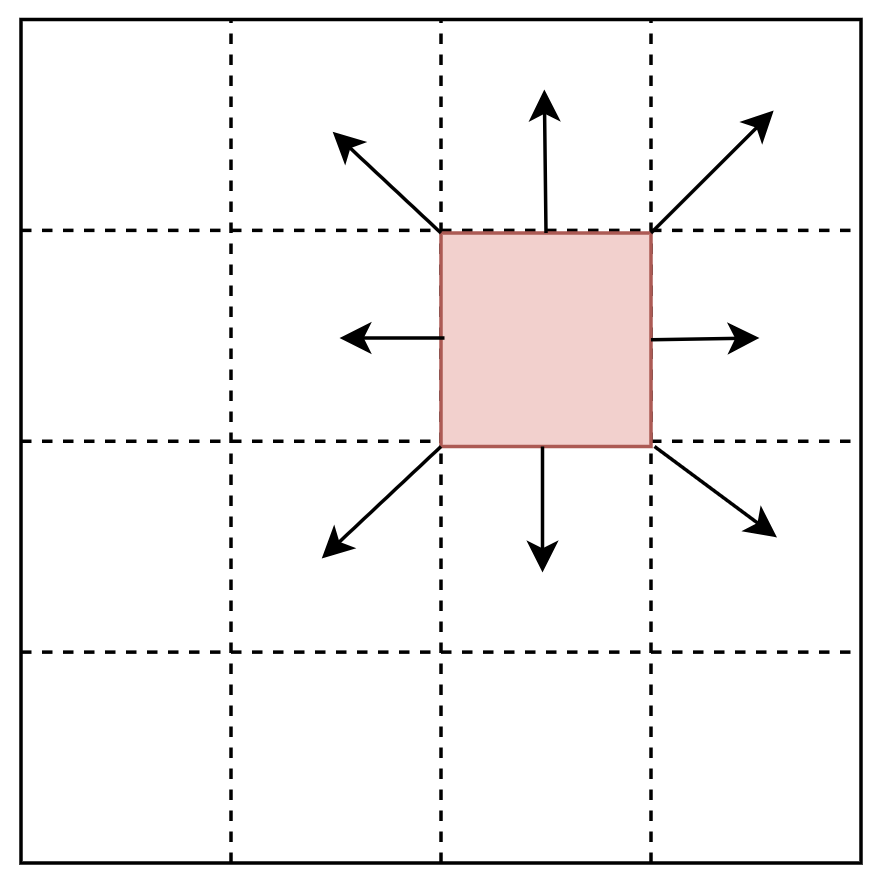
\includegraphics[width=.7\linewidth]{figures/diffusione.png}
    \caption{Diffusione grafica del feromone}\label{fig:diffusion}
\end{figure}
